\input{../YKY-preamble.tex}

\usepackage{color}
\usepackage{mathtools}
\usepackage{hyperref}

% \usepackage[backend=biber,style=numeric]{biblatex}
% \bibliography{../AGI-book}
% \renewcommand*{\bibfont}{\footnotesize}

\usepackage{graphicx} % Allows including images
\usepackage{tikz-cd}
\usepackage{tikz}
\usepackage[export]{adjustbox}% http://ctan.org/pkg/adjustbox
\usepackage{verbatim} % for comments
% \usepackage{newtxtext,newtxmath}	% Times New Roman font

% \numberwithin{equation}{subsection}

\newcommand{\underdash}[1]{%
	\tikz[baseline=(toUnderline.base)]{
		\node[inner sep=1pt,outer sep=10pt] (toUnderline) {#1};
		\draw[dashed] ([yshift=-0pt]toUnderline.south west) -- ([yshift=-0pt]toUnderline.south east);
	}%
}%

\DeclareSymbolFont{symbolsC}{U}{txsyc}{m}{n}
\DeclareMathSymbol{\strictif}{\mathrel}{symbolsC}{74}

\newcommand{\highlight}[1]{\colorbox{pink}{$\displaystyle #1$}}

\newcommand{\emp}[1]{{\color{violet}\textbf{#1}}}
\newcommand*\confoundFace{$\vcenter{\hbox{\includegraphics[scale=0.2]{../2020/../confounded-face.jpg}}}$}
\newcommand{\underconst}{\includegraphics[scale=0.5]{../2020/UnderConst.png}}
\newcommand{\witness}{\scalebox{0.6}{$\blacksquare$}}
% \newcommand{\Heytingarrow}{\mathrel{-}\mathrel{\triangleright}}
\providecommand\Heytingarrow{\relbar\joinrel\mathrel{\vcenter{\hbox{\scalebox{0.75}{$\rhd$}}}}}

\begin{document}

\title{\bfseries\color{blue}{\Huge AGI standard model}\\ --- a proposal}
\author{YKY} % Your name
%\institute[] % Your institution as it will appear on the bottom of every slide, may be shorthand to save space
%{
%Independent researcher, Hong Kong \\ % Your institution for the title page
%\medskip
%\textit{generic.intelligence@gmail.com} % Your email address
%}
\date{\today} % Date, can be changed to a custom date

\maketitle

% \vspace*{0.5cm}
% 多谢 支持 \smiley

\setcounter{section}{-1}
\section{Introduction}

The ``standard model'' is a way of thinking, that may help us better understand the general theory of AGI systems.

The essence of the standard model is just to identify a \textbf{Working Memory} or ``state'' of the AGI system.

\section{Reinforcement learning}

The simplest form of a \textbf{dynamical system}:

When we add an ``action'' or ``control'' variable to it, it becomes the simplest \textbf{control system}:

which is the setting for Dynamic Programming or Reinforcement Learning.

\section{Standard model}

\begin{equation}
\vcenter{\hbox{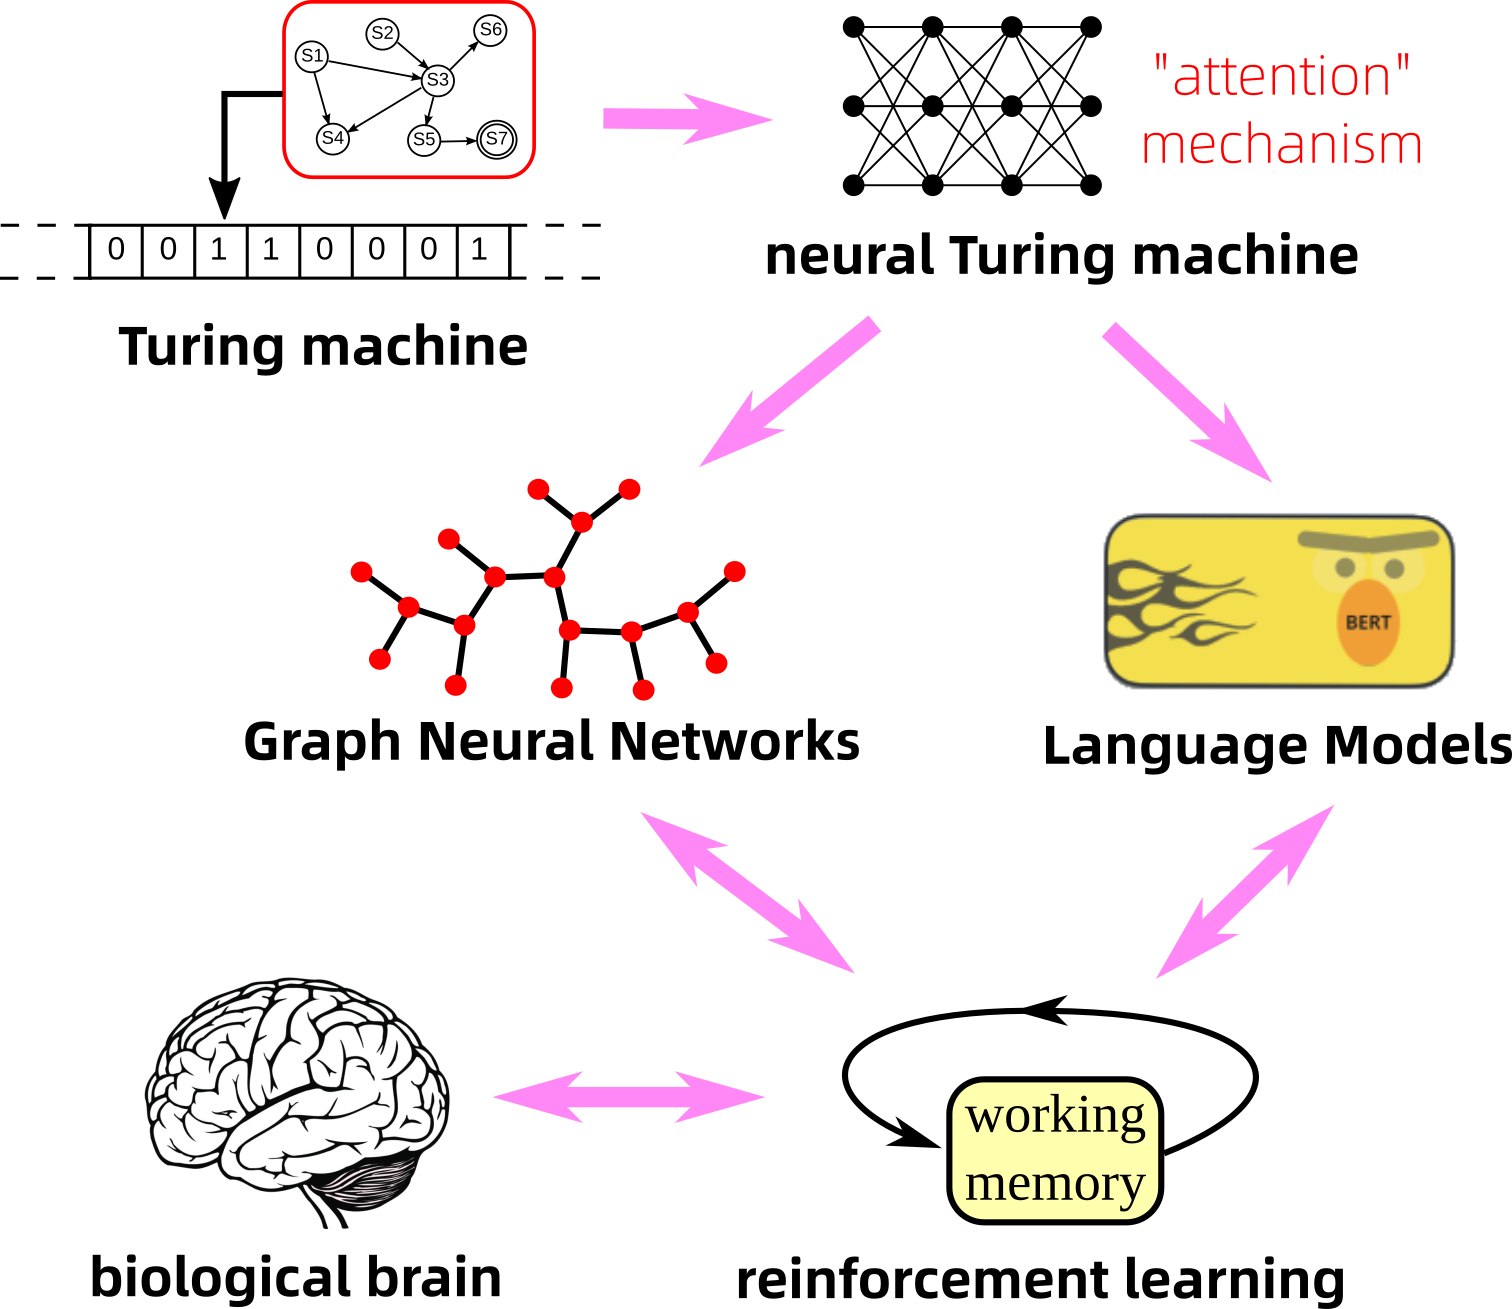
\includegraphics[scale=0.9]{AGI-standard-model.png}}}
\end{equation}

\section{Neural Turing Machine and BERT}

The \textbf{attention mechanism} was first proposed in the ``\textbf{Neural Turing Machine}'' paper by Graves et al.

\section{Relation to the biological brain}

The prefrontal cortex maintains a number of ``thoughts'' with sub-populations or, perhaps, with \textbf{micro-columns}.  These activated sub-populations are in competition with each other, through \textbf{lateral inhibition}.  The thought(s) that win are the thoughts we retain -- they ``make sense''.

\section{Abductive reasoning}

Abductive reasoning is basically just \textbf{bidirectional} inference.

This harks back to the ART (Adaptive Resonance Theory) proposed by Grossberg and Carpenter beginning in the 1980s.

\section{Dealing with assumptions}

An assumption is a $\lambda$-term.  It maps a \textbf{proof witness} to a new proposition.

For example, ``If I play move $x$ now, I will checkmate in 3 moves".






\end{document}
